\section{Cos'è la meccanica quantistica}
La meccanica quantistica è una teoria fisica che descrive il comportamento della materia, delle radiazioni e delle loro interazioni. In particolare studia i fenomeni microscopici e fa parte del \textit{modello standard} (cioè la teoria fisica che descrive tre delle quattro forze fondamentali: interazioni forte, debole, elettromagnetica e tutte le particelle collegate. Essa è quindi incompatibile solo alla relatività generale che spiega la forza di gravità)

\section{Elementi della meccanica quantistica}
\subsection{Dualismo onda-particella}
Nella fisica classica vigevano due blocchi di leggi distinti e apparentemente indipendenti: quelle di Newton, che descrivono i corpi meccanici, e quelle di Maxwell, che invece descrivono i campi elettromagnetici come ad esempio la luce. Quest'ultima era elemento di dibattito in quanto empiricamente con l'esperimento di Young era stato dimostrato che essa è sottoposta ai fenomeni di diffrazione e interferenza: tipici delle onde; ma l'effetto fotoelettrico (emissione di elettroni da parte di una superficie a seguito di un'illuminazione) era spiegabile solo se trattata come insieme di particelle.\\
La meccanica quantistica assume quindi che l'unico modo per spiegare ogni fenomeno fisico è il non limitarsi a considerare la luce \textit{o} onda \textit{o} particella, bensì accettare che essa è entrambi contemporaneamente.\\
Non è comunque solo la luce ad essere soggetta al dualismo, bensì ogni particella: ad esempio nell'esperimento di Zeilinger viene fatto notare come anche i neutroni (normalmente considerati particelle) presentano i fenomeni di interferenza
\subsection{Indeterminazione e casualità}
Per illustrare con miglior chiarezza il concetto partiamo da un paio di esempi.
\subsubsection{Esperimento classico}
Immaginiamo di avere un oggetto, tipo pallina da tennis, che possa essere modellizzato come punto materiale e analizziamo le grandezze fisiche posizione e velocità, ricordandoci che il contesto deve essere controllato in modo che l'esperimento sia ripetibile.\\
All'istante \textit{t=0} la pallina si trova nella posizione \{\textit{x=0,y=0}\} e ad essa imprimiamo una certa velocità. Il moto della pallina sarà parabolico (ricordiamoci che è presente la gravità) come quello mostrato in figura:\\
\begin{center}
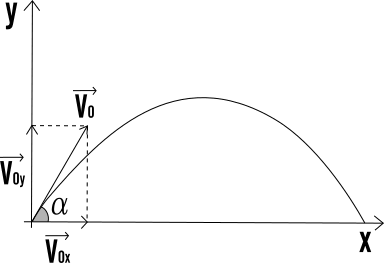
\includegraphics[scale=0.8]{motoParabolico}
\end{center}
La cosa fondamentale che vogliamo evincere da questo esperimento è il fatto che ponendoci nelle stesse condizioni: stessa pallina da tennis, stessa posizione all'istante 0 e stessa velocità; il moto sarà sempre identico e la pallina atterrerà sempre nella stessa posizione. Questo ci fa notare come la natura abbia un comportamento deterministico il che è elemento fondamentale del metodo scientifico: se si ottenessero sempre risultati diversi non si potrebbe fare scienza.
\subsubsection{Esperimento quantistico}
Per questo esempio sfruttiamo il già citato esperimento di Zeilinger:
\begin{center}
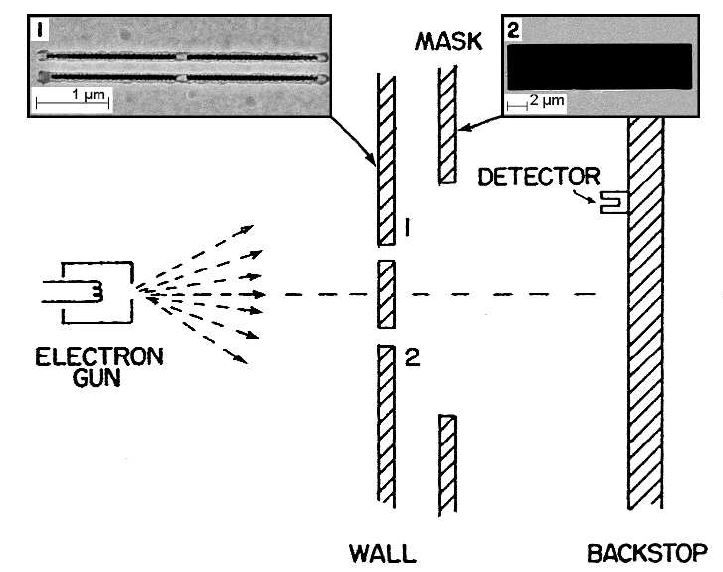
\includegraphics[scale=0.6]{neutronDiffraction}
\end{center}
Come si può vedere dall'immagine l'apparato sperimentale è composto da una pistola per neutroni (c'è scritto elettroni, ma il risultato qualtitativamente non cambia se si usa una particella oppure l'altra); un muro con due fenditure (che sono dell'ordine di grandezza del diametro della particella), una maschera per evitare al più possibile contaminazioni esterne; un muro finale ove con un detector è possibile trovare la posizione in cui il neutrone è arrivato.
Immaginiamo di esaminare un neutrone per volta; esso è preparato sempre alla stessa maniera e sottoposto sempre allo stesso ambiente; ciò che ci si aspetterebbe, ogni volta misuriamo dove si schianta con il muro finale; sarebbe il rilevare sempre la stessa posizione. Questo però non accade, ad ogni iterazione dell'esperimento il risultato è diverso.\\
In conclusione non c'è più determinismo, la natura in realtà è casuale e questo si è appena dimostrato empiricamente.\\
Sorge quindi un dubbio: si può ancora fare scienza? Sembrerebbe di no, e sicuramente il percorso del neutrone non è più deterministico e prevedibile con certezza, però ripetendo l'esperimento un numero molto grande di volte e costruendo un grafico \{numero-neutroni/posizione\} otteniamo sempre un risultato come quello nella figura seguente.
\begin{center} 
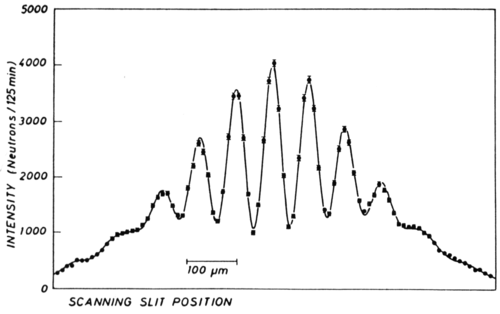
\includegraphics[scale=2.5]{distribuzioneZeilinger} \end{center}
Due sono le osservazioni importanti:
\begin{enumerate}
\item Nel caso in cui si rifacesse tutto da capo otterremmo la stessa identica figura quindi, pur non essendo deterministico un singolo neutrone, lo è la probabilità che in un determinato punto sia rilevato. Diventa quindi possibile "fare scienza" sulle distribuzioni di probabilità di un insieme di neutroni e quindi la descrizione di ognuna delle grandezze fisiche di un sistema quantistico diventa una probabilità.
\item La figura che si è andata a creare corrisponde esattamente a una figura di interferenza a due fenditure, confermando (come già detto) il dualismo onda-particella
\end{enumerate}
\subsubsection{Limite classico della meccanica quantistica}
A questo punto è necessario chiedersi come mai i modelli matematici applicati a corpi microscopici siano radicalmente diversi da quelli che compongono la fisica classica; in fondo ogni oggetto macroscopico è infine composto da particelle fondamentali che seguono la meccanica quantistica.
Le soluzioni a cui si può arrivare sono molteplici, ma tutte non esaustive, le quali hanno addirittura aperto un dibattito filosofico. Qui però rimaniamo all'interno dell'\textit{interpretazione di Copenaghen}, la teoria più importante. Innanzitutto dato che un corpo macroscopico è formato da un numero enorme di particelle può valere la \textit{legge dei grandi numeri} e quindi ciò che si manifesta non è altro che la "vittoria" dell'evento più probabile. Poi è possibile risalire ad alcune equazioni classiche da quelle quantistiche ponendo $\hbar$ $\to$ 0 allo stesso modo di come le trasformazioni di Lorentz diventano quelle di Galilei se \textit{c}$\to 0$.\\
$\hbar$ è la costante di Planck ridotta, ma non essendo lo scopo dell'elaborato analizzare la matematica dietro la meccanica quantistica l'argomento non verrà approfondito.\\
Rimangono però problemi legati al fenomeno dell'\hyperref[sec:entanglement]{entanglement} che affronteremo fra poco
\subsection{La sovrapposizione}
Come detto ogni grandezza fisica viene quindi definita e trattata come una distribuzione di probabilità, vediamo in questa sezione cosa significa un po' più nel dettaglio.\\
Come esempio prendiamo lo spin di un elettrone in quanto può assumere solamente due valori: $\frac{1}{2}$ e -$\frac{1}{2}$ al contrario di tante altre grandezze fisiche che, come ad esempio la posizione, possono assumere infiniti valori continui
\subsubsection{Gli autostati}
Cominciamo a vedere la situazione più semplice: lo spin ha probabilità 1 (o 100\%) di essere $\frac{1}{2}$ e probabilità 0 di essere -$\frac{1}{2}$.\\
In questo caso si dice che la grandezza fisica $\textit{spin}$ è in un $\underline{autostato}$ e il valore assunto ($\frac{1}{2}$) è un $\underline{autovalore}$. Quello che accade quindi è che preparando l'esperimento sempre allo stesso modo l'osservazione dello $\textit{spin}$ produrrà sempre lo stesso risultato.\\
Per estensione qualsiasi grandezza fisica cui la misura di un determinato sistema produce sempre lo stesso risultato (tenendo ovviamente conto degli errori) è un $\underline{autostato}$ indipendentemente da quanti valori la grandezza avrebbe potuto assumere.
\subsubsection{La sovrapposizione}
Quando più valori hanno probabilità non nulla di essere presenti si dice invece che il sistema, per quella grandezza fisica, è in uno stato di $\underline{sovrapposizione}$ (o superposizione dall'inglese $\underline{superposition}$). Ad esempio nel caso la probabilità di ottenere $\frac{1}{2}$ è 0.5 e di -$\frac{1}{2}$ è 0.5 oppure $\frac{1}{2}$: 0.3 e -$\frac{1}{2}$: 0.7 il sistema è in $\underline{sovrapposizione}$. Da ricordare comunque che la somma di tutte le probabilità deve essere sempre 1. Questa però è una semplificazione in quanto in realtà in meccanica quantistica è necessario esprimere le probabilità di ogni valore con numeri complessi rendendo quindi modelli matematici piuttosto complicati, soprattutto in caso di grandezze fisiche continue. A riguardo se ne riparlerà nel capitolo Bit e Qubit nella descrizione di un computer quantistico.\\
Esistono vari modi per produrre uno stato di sovrapposizione con determinate distribuzioni di probabilità in laboratorio, vedremo un esempio nella sezione successiva parlando del principio di Heisenberg
\subsubsection{Vero stato della materia}
Prima di passare oltre è importante fare il punto su una questione:
ogni elemento della meccanica quantistica che abbiamo finora esaminato ( ugualmente tutti gli altri concetti); quindi il $\underline{dualismo}$, la $\underline{sovrapposizione}$ ecc. non esistono solo in quanto gli apparati sperimentali non sono abbastanza precisi o non si prendono in considerazione alcune variabili; ma è proprio la realtà che mostra comportamenti quantistici contradditori ad una mentalità classica.
\subsection{La misura}
Nella meccanica quantistica la misura copre un aspetto particolare, piuttosto diverso dalla misura classica.
Infatti classicamente è quasi sempre possibile valutare lo stato di un sistema senza perturbarlo negli aspetti interessati; quando non è così la causa sono gli strumenti di misura oppure la perturbazione è determinata e si può risalire matematicamente all'informazione cercata.\\
In meccanica quantistica invece la misura perturba sempre il sistema e in particolare rompe lo stato di $\underline{sovrapposizione}$ e lo rende un $\underline{autostato}$ presentando di uno qualsiasi degli $\underline{autovalore}$, ma secondo la distribuzione di probabilità della sovrapposizione.
Questo è molto importante in quanto la trasformazione applicata dalla misura non è prevista dalle varie equazioni (ad esempio quella di Schrodinger) per la trasformazione di un sistema quantistico e non ha una spiegazione logica; diventando quindi il punto di partenza per teorie esotiche come il multimondo (in cui in più universi paralleli si presentano i diversi $\underline{autovalori}$)
\section{Conseguenze e altri concetti}
\subsection{Indeterminazione di Heisenberg}
Ragionando sulla misura della posizione di un elettrone Heisenberg arrivò ad una legge incredibilmente importante per la relazione di due grandezze fisiche quantistiche:\\
Per misurare la posizione di un elettrone è necessario illuminarlo con un fotone, e in particolare più bassa è la lunghezza d'onda più la misura sarà precisa; ma così aumenta anche l'energia trasportata e quindi la perturbazione della sua velocità. In conclusione più è la precisione con cui si conosce la posizione (e quindi si tende ad un $\underline{autostato}$) meno è la precisione con cui si conosce la velocità e viceversa. Heisenberg scrive quindi questa disequazione:
\begin{center} \begin{Large}
 $\sigma(\textit{p}) \cdot \sigma (\textit{x}) \geq \frac{\hbar}{2}$ \end{Large} \end{center}
in cui $\sigma(\textit{a})$ è la diviazione standard della grandezza fisica \textit{a}; \textit{p} è la quantità di moto (massa per velocità) e \textit{x} la posizione.\\
Questa disequazione vale per moltissime coppie di grandezze fisiche; tra le più famose e interessanti (oltre a quantità di moto e posizione) sono energia-tempo e spin lungo direzioni perpendicolari.\\
Una grandezza fisica è quindi determinata al massimo in modo inversamente proporzionale all'altra. In questo modo è semplice costruire in laboratorio un sistema con una grandezza fisica in $\underline{sovrapposizione}$: basta misurare la grandezza che sta in coppia.\\
Conseguenze di questo principio sono molteplici, ad esempio l'effetto Zenone per il quale è possibile bloccare l'evoluzione nel tempo di un sistema fisico continuandolo ad osservare.\\
Possiamo vedere nella pratica quanto il principio di Heisenberg si allontani dalla fisica classica con questo esperimento:\\
Si parte da un insieme di particelle di cui non si sa nulla riguardo lo spin; si posiziona un apparato di Stern-Garlach come quello in figura (esso divide le particelle secondo lo spin della direzione in cui sono posizionati) lungo una determinata direzione (che può essere chiamata \textit{x}); scopriamo che metà hanno spin positivo e metà negativo e decidiamo di scartare queste ultime.
\begin{center}
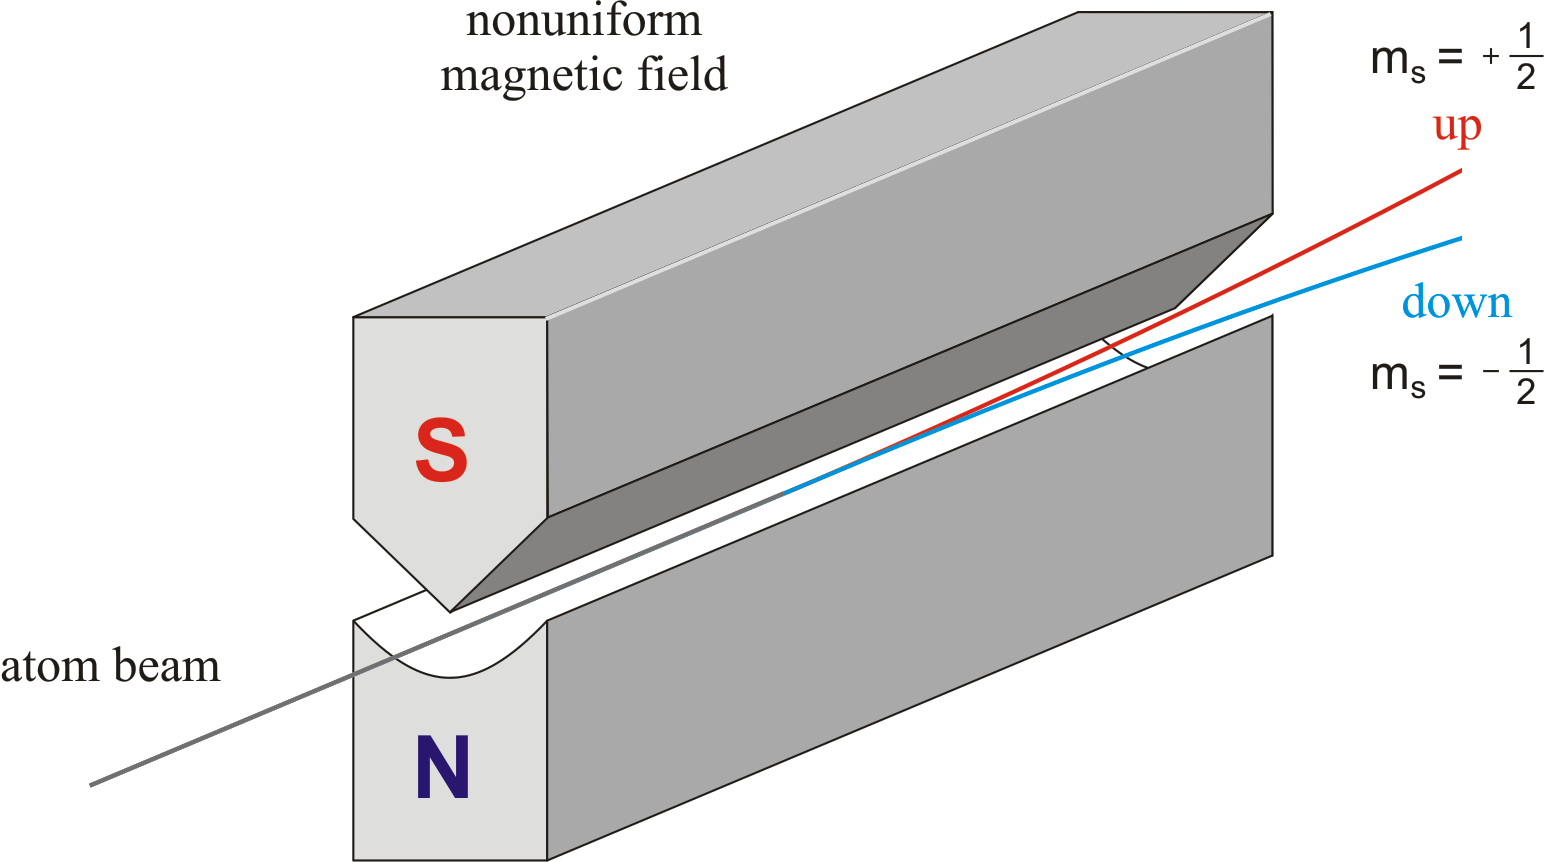
\includegraphics[scale=0.8]{stern-gerlach}
\end{center}
Ora siamo sicuri che lungo \textit{x} ogni particella ha spin positivo. Passiamo queste in un altro apparato di  Stern-Garlach lungo una direzione perpendicolare a \textit{x} chiamata \textit{z}; anche qui notiamo che metà hanno spin positivo e metà negativo e decidiamo nuovamente di tenere solo quelle a spin positivo.\\
Per come è costruito l'apparato sperimentale esso non interagisce in alcun modo con le particelle se non deviandone il moto e sicuramente non può modificare lo spin di queste ultime. Ci si aspetterebbe quindi che alla fine abbiamo solo particelle con spin positivo sia lungo \textit{x} che lungo \textit{z}. Se riposizioniamo però un apparato di Stern-Gerlach lungo \textit{x} si nota che solo la metà hanno spin positivo.\\
Questo ha senso solo nell'ottica della meccanica quantistica e del principio di Heisenberg; infatti nel momento in cui sono state selezionate le particelle lungo \textit{z} l'indeterminazione lungo essa è nulla e quindi lungo le direzioni perpendicolari (tra cui \textit{x}) deve essere infinita; cioè ogni valore è equiprobabile e perciò metà hanno spin positivo e metà negativo.
\subsection{Entanglement}
\label{sec:entanglement}
Nel 1935 Einstein (insieme a Podolski e a Rosen) per cercare di dimostrare l'incompletezza dei modelli probabilistici tipici della meccanica quantistica propone un esperimento mentale poi denominato \textit{Argomento EPR}.
In esso propone un sistema composto di due particelle che hanno interagito tra loro in modo tale che il momento angolare complessivamente nullo, e dato che singolarmente ogni particella non lo ha nullo le due devono averlo opposto: $p_A=-p_B$(Vedere figura)
\begin{center}
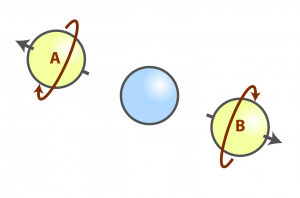
\includegraphics[scale=0.9]{epr}
\end{center}
\textit{A} e \textit{B} sono le due particelle e la sfera al centro rappresenta l'origine.\\
Dal momento in cui le due particelle non hanno più interazioni vale il principio di conservazione del momento totale e quindi sia \textbf{posizione che momento devono rimanere simmetrici rispetto all'origine}.\\
Questo vincolo è chiamato stato \underline{\textit{entangled}} (termine coniato successivamente da Schr\"{o}dinger).\\
L'analogo nella meccanica classica è un fenomeno che non pone nessun dubbio, ma in quantistica le grandezze fisiche sono intrinsicamente aleatorie il che pone conseguenze problematiche.
Ripetendo l'esperimento più volte i valori misurati sono sempre diversi, ma misurando le due particelle essi sono comunque opposti; le possibili spiegazioni sono solamente due:
\begin{enumerate}
\item i valori misurati non sono in realtà casuali, ma prederminati in fase di preparazione dell'esperimento; sono presenti variabili non note che fanno ottenere valori sempre diversi, ma comunque in modo determinato.
\item i valori sono genuinamente casuali e si manifestano solo all'atto della misura, ma esiste una comunicazione istantanea che alla misura su una particella modifica lo stato dell'altra per far ottenere con certezza il valore opposto.
\end{enumerate}
In quegli anni è scientificamente accettata e sufficientemente dimostrata la \textit{relatività speciale}, la quale pone però un limite alla velocità massima raggiungibile (equivalente a $\underline{c}$); una comunicazione istantanea non può quindi esistere.\\
La conclusione che ne trae Einstein è perciò il fatto che esistano variabili "nascoste" e l'interpretazione non deterministica è sbagliata.\\
Però l'esperimento EPR ha altre conseguenze; in particolare la \textit{\underline{disuguaglianza di Bell}} in cui viene fatto notare che, in caso di variabili nascoste o di casualità intrinseca la probilità cui alcuni valori si sarebbero manifestati è diversa. Andando quindi a compiere un esperimento e verificare le probibilità di comparsa di alcuni valori è possibile capire quale delle due spiegazioni è corretta.\\
Dagli anni 70-80 fu finalmente possibile effettuare versioni modificate di EPR che tutte però sottoposte alla \textit{\underline{disuguaglianza di Bell}} confermarono che la casualità è intrinseca ed esiste in effetti una comunicazione istantanea. Essa non è però forzatamente contro la teoria della relatività speciale in quanto le comunicazioni istantanee sono di valori casuali e non esiste alcun modo di inviare un messaggio scelto più velocemente di \textit{c}.
\subsubsection{Il gatto di Schrodinger: vivo o morto?}
A riguardo della meccanica quantistica e dell'entanglement è famosissimo il paradosso di Scr\"{o}dinger, il quale fa risaltare il problema della distinzione tra microscopico e macroscopico, ciò che è sottoposto ai fenomeni quantistici e cosa no.\\
Nel paradosso viene proposto un esperimento:\\
Si ha una scatola all'interno della quale non è possibile fare alcuna misura; essa contiene un atomo radioattivo; un contatore Geiger connesso ad una bottiglietta di cianuro e se l'atomo decade la bottiglietta viene rotta. Nella scatola c'è poi un gatto.\\
In questo sistema il decadimento radioattivo è un fenomeno quantistico e l'atomo è in stato di sovrapposizione: è quindi sia decaduto che no fino a che non si compie una misura, ma allora il contatore Geiger ha sia rotto la bottiglietta che no e il gatto è sia vivo che morto finchè l'atomo non viene osservato e cade in un autostato.